\documentclass[12pt,letterpaper,twoside]{article}
\usepackage{../cme211}

\usepackage{atbegshi}% http://ctan.org/pkg/atbegshi

\begin{document}
\title{Lecture 7: Data Representation, Numerical Python\vspace{-5ex}}
\date{Fall 2020}
\maketitle

{\footnotesize
\paragraph{Topics Introduced:} Binary vs. Decimal systems, simplified
concepts of computer architecture including hierarchical memory and
arithmetic logic units, representation of integers, strings, and
floating point types, as well as \texttt{numpy}.
}
\vspace{-3ex}
\section{Representation of Data}

\subsection{Computer Representation of Integers}
Computers represent and store everything in
\href{https://en.wikipedia.org/wiki/Binary_number#Binary_counting}{\emph{binary}},
which is a base 2 number system. How is this different from what we
are familiar with in our base-10 (i.e. decimal) number system?

\begin{itemize}
\item Decimal counting uses the symbols 0-9.
\item Counting starts by incrementing the least-significant
  (rightmost) digit.

\begin{verbatim}
000, 001, 002, ..., 009
\end{verbatim}
\item When we exhaust the set of available symbols, we realize a type
  of overflow, in which the least-significant digit is reset to zero
  and the next digit of higher significance is incremented.

\begin{verbatim}
010, 011, 012, ..., 099
\end{verbatim}

\item We repeat this process of allowing for overflow with each digit
  of significance.

\begin{verbatim}
100, 101, 102, ...  
\end{verbatim}
\end{itemize}

To be formal, you can think of the integer $d_m
d_{m-1} \ldots d_1 d_0$ as being equivalent shorthand for
\[
  d_0 \times 10^0 + d_1 \times 10^1 + \ldots + d_{m-1} \times 10^{m-1}
  + d_m \times 10^m,
\]

where each symbol $d_i$ can take on a single value from the set $\{0,
1, \ldots, 9\}$.
\href{https://en.wikipedia.org/wiki/Binary_number#Binary_counting}{Counting
  in binary} is no different, sparing the fact that our set of
symbols is reduced to have cardinality two, i.e. the atomic elements are
\href{https://en.wikipedia.org/wiki/Bit}{\emph{binary digits} (bits)}
which can be toggled between zero or one.

\begin{centering}
\begin{table}[h]
  \hspace{-6ex}
\begin{tabular}{l r r r r r r r r r r r r r r r r}
  Decimal & 0 & 1 & 2 & 3 & 4 & 5 & 6 & 7 & 8 & 9 & 10 & 11 & 12 & 13
  & 14 & 15 \\
  Binary & 0 & 1 & 10 & 11 & 100 & 101 & 110 & 111 & 1000 & 1001 &
                                                                   1010
                                                       & 1011 & 1100 &
                                                                       1101
  & 1110 & 1111
\end{tabular}
\caption{A table describing how values can be equivalently represented
  in either a decimal or a
  binary number system.}
\end{table}
\end{centering}

To be formal, we can think of the integer $b_m b_{m-1} \ldots b_1 b_0$
as being equivalent shorthand for
\[
  b_0 \times 2^0 + b_1 \times 2^2 + \ldots + b_{m-1} \times 2^{m-1} +
  b_m \times 2^m
\]
where here we are using $b_i$'s to remind ourselves that each symbol
is a binary digit taking on only one of two values. Notice that other
than the set of symbols changing, the \emph{base} has changed as well,
from 10 to 2. Once you learn these basics, \href{https://en.wikipedia.org/wiki/Binary_number#Conversion_to_and_from_other_numeral_systems}{converting between numeral
systems} is easy.

There are 8 bits in a
\href{https://en.wikipedia.org/wiki/Byte}{byte}. Depending on the
computer architecture, a
\href{https://en.wikipedia.org/wiki/Word_(computer_architecture)}{word}
could be 4 or 8 bytes.

\subsubsection{Simplified Model of Computer}
Where are our data stored on a computer? How is it operated on?
A typical computer will have a memory hierarchy to facilitate
long-term storage (e.g. hard-disk), medium-term storage (RAM), and
short-term storage (cache). We present a simplified computer
architecture below, which does not picture long-term storage.

\begin{figure}[h]
\centering
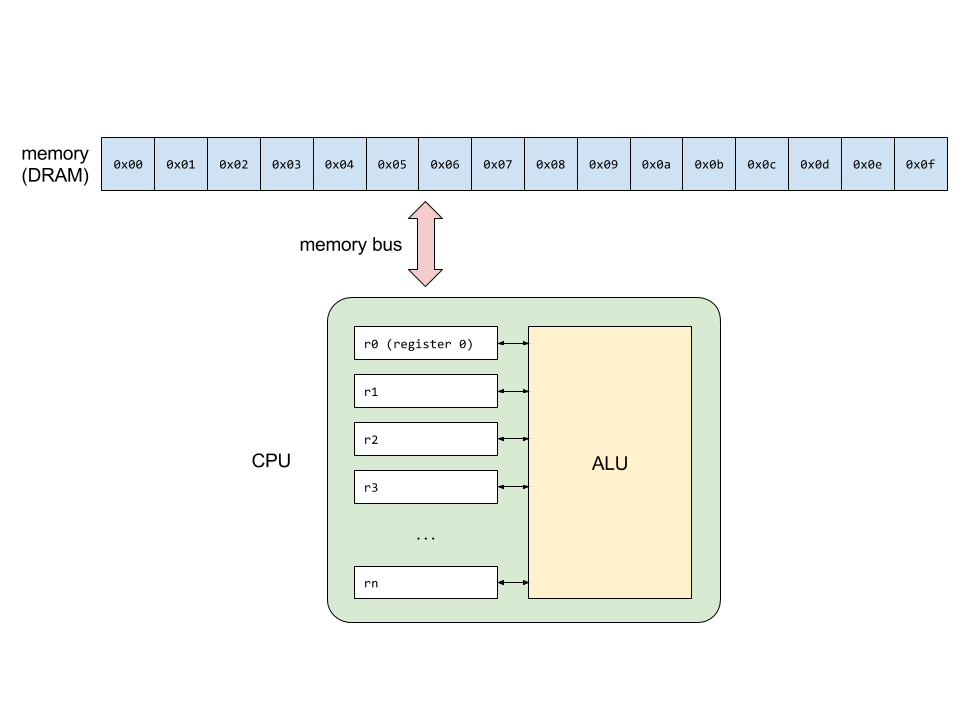
\includegraphics[scale=0.45]{fig/model-computer.png}
\caption{\footnotesize We take a simplified view of a computer architecture. In
  particular, we show the relationship between
  \href{https://en.wikipedia.org/wiki/Computer_data_storage\#Primary_storage}{primary
    memory}
  (e.g. \href{https://en.wikipedia.org/wiki/Random-access_memory}{RAM})
  and a
  \href{https://en.wikipedia.org/wiki/Central_processing_unit}{CPU}. The
  CPU contains (i)
  \href{https://en.wikipedia.org/wiki/Arithmetic_logic_unit\#Functions}{arithmetic
    logic units} which take two inputs and produce a single output
  (think of the operators \texttt{+}, \texttt{-}, \texttt{\&}, and \texttt{|}) and (ii)
  \href{https://en.wikipedia.org/wiki/Processor_register}{registers}
  which can (very quickly) store inputs for ALU operations and hold corresponding outputs.}
\end{figure}

\subsubsection{Common Prefixes}
There can be some confusion here depending on the context of
usage. That is, in the context of networking and storage, the prefixes
\texttt{kilo}, \texttt{mega}, \texttt{giga}, \texttt{tera},
\texttt{peta}, and \texttt{exa} all use base 2. However, many other
contexts speak in base 10, e.g. cpu-frequencies and ethernet speeds.

The prefix
\href{https://en.wikipedia.org/wiki/Kilobyte#Definitions_and_usage}{kilo}
always means one-thousand in the prefix of an
\href{https://en.wikipedia.org/wiki/International_System_of_Units#Prefixes}{International
  System of Units}. However, since we understand the difference
between a \texttt{bit} and a \texttt{byte}, we can now understand that
there is a difference between a \texttt{kilobyte} (denoted by \textbf{kB}) and
a \emph{kibibyte} (denoted by \textbf{KiB}). The former is 1,000 bytes, i.e. 8,000
bits, whereas the latter is 1,024 bytes. i.e. 8,192 bytes.
We ask that you remember that there is a big difference between these
terms, but not necessarily that you remember the exact terminology or
symbols used to denote each. Wikipedia has a nice table demonstrating
how binary and decimal systems use
\href{https://en.wikipedia.org/wiki/Orders_of_magnitude_(data)}{different prefixes across orders of magnitude}. 

\subsubsection{Computer Storage of an Integer}
At the hardware level computers \textbf{don't} do variable length
representations of numbers. I.e. although we may use a variable length
representation, writing $4_{10} = 100_2$, or $73_{10} = 1001001_2$,
computers often use a fixed width storage for numeric types.

\begin{figure}
\centering
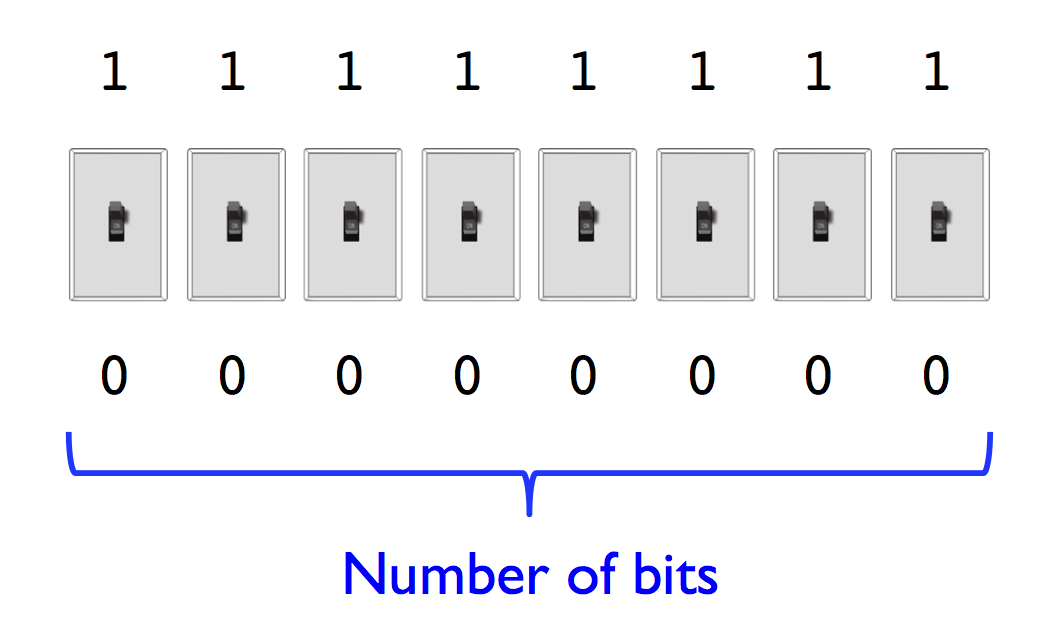
\includegraphics[scale=0.35]{fig/bits.png}
\caption{\footnotesize We can think of a (fixed-width) sequence of bits as a panel
  of lightswitches, each capable of being toggled on or off. }
\end{figure}

At the hardware level computers typically handle integers using 8, 16,
32, or 64 bits, depending on the architecture.

\vspace{-3ex}
\paragraph{Number of Representable Values Given $n$ Bits}
Realize that for a sequence of \texttt{n} bits, it may take on exactly
$2^n$ different values.
This dictates the range of what can be represented with a fixed number
of bits. Some common bounds we run into are.
\begin{verbatim}
2^8  = 256
2^16 = 65536                   ~(65 thousand)
2^32 = 4294967296              ~(4 billion)
2^64 = 18446744073709551616    ~(18 followed by 18 zeros)
\end{verbatim}

I.e. when we went from 32-bit machines to 64-bit machines, we didn't
just double their capacity. The latter can store
10 orders of magnitude more information (in each register), akin to allowing 10
more decimal digits to be represented. This follows from the fact that

$$
\log_{10}(2^{64} / 2^{32}) = 64 \log_{10}(2) - 32 \log_{10}(2) = 32
\log_{10}(2) \approx 10.
$$

\vspace{-3ex}
\paragraph{Using a Sign Bit to Store Negative Integers}
The idea is to simply use one bit to store the sign of a value, and
the remaining bits to track magnitude.
This reduces the range of the magnitude from $2^n$ to
$2^{n-1}$. E.g. suppose that we have a
\href{https://en.wikipedia.org/wiki/Nibble}{nibble} to work with,
i.e. four bits. We can represent the values
$\pm 4$ as indicated at the right of each statement.

\begin{align*}
  \texttt{4}_{10} &= \hspace{30pt} (\texttt{100})_2 &&\leadsto (\texttt{0100}) \\
  -\texttt{4}_{10} &= -1 \times (\texttt{100})_2 &&\leadsto (\texttt{1100})
\end{align*}

\paragraph{Offset: An Unconventional Way to Represent Negative Values}
Another idea instead of using a sign bit is to simply
apply an offset or bias to reinterpret the conversion between binary
and decimal. One example may look as follows.

\begin{figure}[h]
\centering
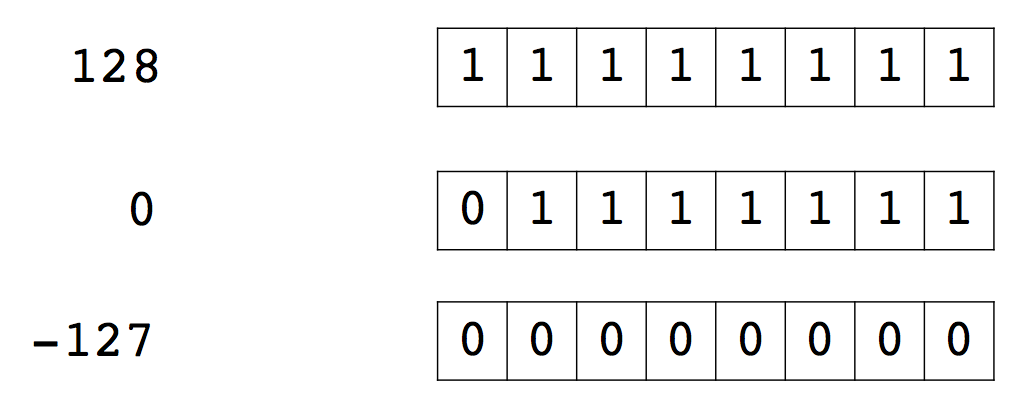
\includegraphics[scale=0.5]{fig/sign-offset.png}
\caption{\footnotesize Suppose we have a byte or eight bits. There are $2^8
= 256$ values that can be represented by such a sequence of
bits. Centering the number of distinct values around the integer zero,
we find that we can represent the set of values $\{-127, \ldots, 0, 1,
\ldots, 128\}$. If we use an offset method for representing integers,
then we may decide to set the sequence of eight bits as all zero's to
represent the minimum value $-127$, and from here we can apply the
usual rules of carry-over/overflow to count our way up to $128$.}
\end{figure}

Again, whether we use the idiom of a sign-bit or if we apply an
offset, either way we effectively reduce the range of the magnitude of
integers allowed. Intuitively, whether or not a number is positive or
negative should \emph{require one unit of information}.

Many programming languages support unsigned integers. Although
Python itself does not have \textbf{unsigned integers}, but \texttt{numpy} does.
A programmer can use this to their advantage by expanding the effective range available
if negative numbers don't need to be stored.
But! With any fixed-storage representage of a real number, we must beware.

\begin{itemize}
\item Attempting to assign a value greater than what can be represented by
the data type will result in \href{https://en.wikipedia.org/wiki/Integer_overflow}{\emph{overflow}}.
Overflow tends to cause \emph{wraparound}, e.g.~if adding
together two signed numbers causes overflow the result is likely to be
a negative number.

\item Attempting to assigning a value less than what can be represented by
the data type will result in
\href{https://en.wikipedia.org/wiki/Arithmetic_underflow}{\emph{underflow}}.\footnote{We
  can try to fill the underflow gap using \href{https://en.wikipedia.org/wiki/Denormal_number}{denormal numbers}.}
  Underflow can cause a division by zero error, for example, if we
  were to scale by the difference between two quantities
  $\frac{1}{b-a}$ where $a \neq b$ but $a \approx b$. 
\end{itemize}

\subsubsection{Range of Integer Types}
For a fixed number of bits, if we choose to represent sequential
integers centered around zero we must make a decision on boundaries.
E.g. with eight bits, one can store
$2^8 = 256$ unique different bit-sequences (or values), where we have the choice of
either being able to represent the values $\{-128, \ldots, 127\}$ or
$\{-127, \ldots, 128\}$. In general, an $n$-bit representation of an
integer stores the values in the set
\[
  \{\underbrace{-2^{n-1}, \ldots, -1}_{2^{n-1} \textrm{ elements}}, \underbrace{0,
  \ldots, 2^{n-1} - 1}_{2^{n-1} \textrm{ elements}}\}.
\]

\paragraph{Integers in Python}

In Python 3, values of type \texttt{int} may have unlimited
range.\footnote{Python 2 had both fixed size integers (with type \texttt{int}) and
  variable width integers (with type \texttt{long}).}
This is quite nice, and perhaps surprising if you come from
other programming languages.

\begin{python}[basicstyle=\small]
i = 52**100
print(type(i))   # <class 'int'>
print(i)         # This is beyond the 64-bit integer range.
\end{python}

The module \texttt{numpy} supports \emph{only} fixed-width integers
for reasons that relate to both performance and storage.

\subsection{Strings}

\subsubsection{ASCII}
American Standard Code for Information Interchange (ASCII) is
typically used to encode text information.
Characters, numbers, symbols, etc. are encoded using 7 bits (although
on modern computers they would typically use 8 bits).

E.g. \texttt{A} maps to $\texttt{(1000001)}_2 = (65)_{10}$,
and \texttt{B} maps to $\texttt{(1000010)}_2 = (66)_{10}$.

Default Python 2 string is ASCII. Possible to get \href{https://en.wikipedia.org/wiki/Unicode}{Unicode} strings with \newline
\texttt{s\ =\ u\textquotesingle{}I\ am\ a\ unicode\
  string!\textquotesingle{}}.

\subsubsection{Why Not ASCII All The Way Down? Motivating UTF-8}
\paragraph{For English, A Single Byte Suffices}
The English language has
26 letters (52 if we include casing). If we throw in punctuation and
digits 0-9, we realize that we have more than 64 unique characters to
represent. I.e. we need at least 7 bits. Since computers are more
efficient at processing bit sequences aligned a particular way, many
implementations use 8-bits for an ASCII set. 

\paragraph{For Languages with Ideographs, Require 2 Bytes}
But what about other languages? Chinese,
Japanese, and Korean have somewhere between $2^8$ and $2^{16} - 1$
unique characters, whence we
require a two-byte
sequence to store each character in these languages.
So, different languages (or regions) require different
\href{https://en.wikipedia.org/wiki/Character_encoding#Common_character_encodings}{\emph{character
    encodings}} to map symbols (text) to bit-sequences.

\paragraph{For World of All Languages, (naively) Require 4 Bytes}
But what about
the world wide web? The number of unique characters across all
languages exceeds $65,535$, whence we require strictly more than
two-bytes to encode any character coming from any language in the
world. Sticking with powers of two, we'll use four-bytes. But all of a
sudden, we realize how expensive this has become; any given language
only requires one or at most two bytes per character, but we're using
double that.

The advantage to UTF-32 (the 4-byte unicode encoding) despite it being
costly in terms of storage is that because each character is
represented as a fixed width sequence of bits, we can slice into
strings in constant time. I.e. looking up the $n$th character in a
string is easy, we simply look up where the object lives in memory and
jump $n$ characters forward in memory, where each character
corresponds to exactly 32-bits.

\paragraph{Using a Variable Length Encoding $\leadsto$ Efficiency}
Alas, we've followed Mark Pilgrim's motivation of UTF-8
\href{http://histo.ucsf.edu/BMS270/diveintopython3-r802.pdf}
{as per Chapter 4 of ``Dive Into Python''}. UTF-8 is a \emph{variable length encoding}.
The implication is that the set of ASCII characters each
requires only a single byte per character. Latin characters such as
{\"a} and {\~n} may require two bytes per character, Chinese
characters may involve three bytes, and rarely used characters require
four bytes. However, since each character requires a different
number of bits, we can \emph{no longer} jump to the $k$th character of a string with
$O(1)$ work; we're relegated to inspecting the first $k-1$ characters
to find out where in the bit-sequence the $k$th character is represented.

\paragraph{Default String Encoding in Python is UTF-8}
Default string encoding in Python 3 is
\href{https://en.wikipedia.org/wiki/UTF-8}{UTF-8}.
The change from ACSII to Unicode between Python 2 and 3 caused major
headaches for Python community.
The fact that each character of text may take from
1 to 4 bytes is nice in that the 1-byte codes
correspond to ASCII characters, which makes UTF-8 backwards
compatible with ASCII. Currently,
UTF-8 encodes a total of 1,112,064 characters, which is enough to represent
the majority of human character systems.

\subsection{Floating Point Representation of Numeric Values}
How do we represent a floating point value using bits?

\begin{figure}[h]
\centering
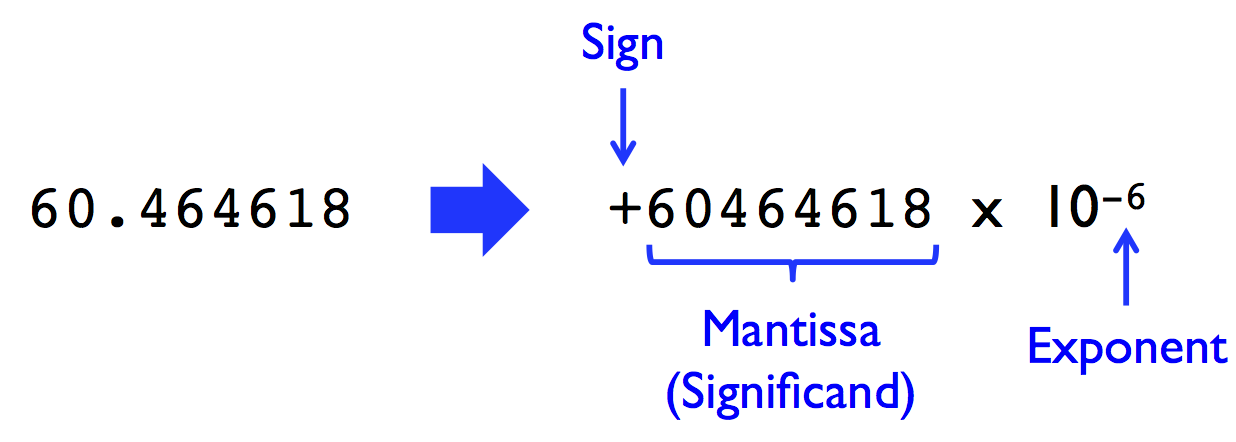
\includegraphics[scale=0.45]{fig/float.png}
\caption{\footnotesize A representation of a decimal value that is broken down into
  three pieces: (i) a sign bit, (ii) a fractional component, and (iii)
  an exponent indicating the magnitude of rescaling. This is a generic
  recipe for approximating real numbers using a finite set of bits.}
\end{figure}


\subsubsection{Floating Point Standard}
\href{https://en.wikipedia.org/wiki/IEEE_754}
{IEEE (Institute of Electrical and Electronics Engineers) 754} is the
technical standard for floating point used by all modern processors
The standard also specifies things like rounding modes, handling overflow,
divide by zero, etc. 

\begin{figure}[h]
\centering
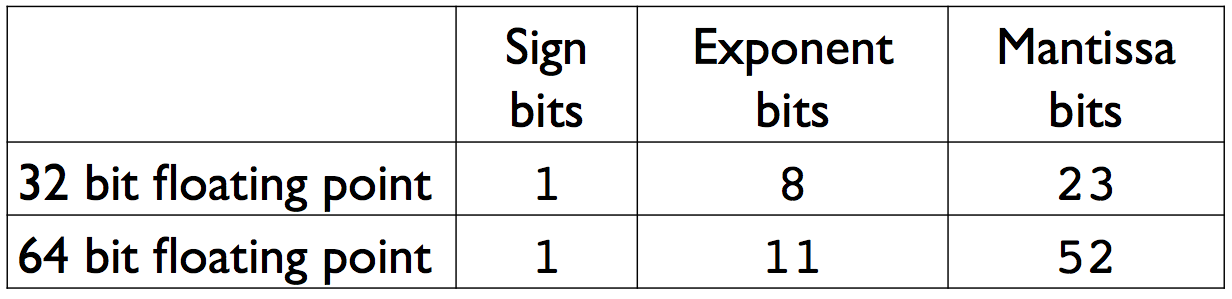
\includegraphics[scale=0.4]{fig/float-table.png}
\caption{\footnotesize 32 vs. 64-bit floating point formats.
  In moving from 32-bit to 64-bit standards, IEE
  increased the number of bits allocated to the mantissa significantly
  more than they did the exponent: with 11-bits for the
  exponent, we can represent $2^{11} = 2,048$ different values of
  exponents. We center these exponents around zero using a
  \href{https://en.wikipedia.org/wiki/Exponent_bias}{exponent bias},
  such that we can store exponents in the range $\pm 2^{10}$. But
  these are exponents, i.e. they are used to raise our base to a
  specified power. That's an astronomically
  large rescaling.}
\end{figure}

\begin{figure}[h]
  \centering
  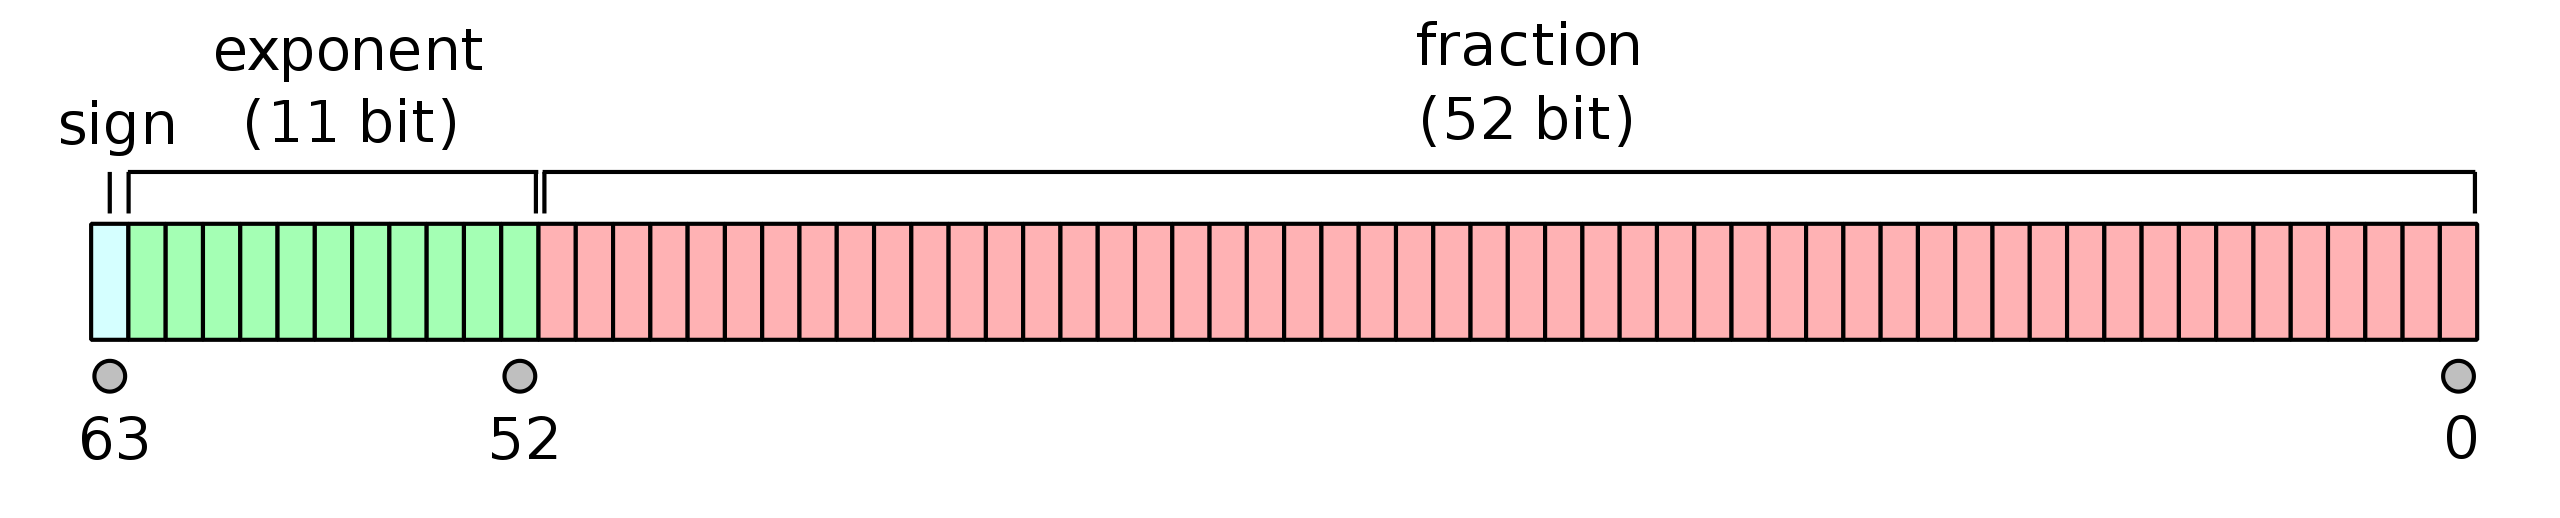
\includegraphics[scale=0.1]{fig/IEEE_754}
  \caption{\footnotesize A visual layout of the 64 bit representation used to store
    a floating point value. We have 1 sign bit, 52 mantissa
(significand, fractional) bits, and 11 exponent bits. Source: \href{https://en.wikipedia.org/wiki/Double-precision_floating-point_format}{Wikipeda}.}
\end{figure}

Symbolically, 

\begin{align*}
  (-1)^{\textrm{sgn}} \underbrace{\left(1 + \sum_{i=1}^{52} b_{52-i} 2^{-i}
  \right)}_{= \left(1.b_{51} b_{50} \ldots b_0\right)_2} \times 2^{\textrm{exp} - 1023}
\end{align*}

where the exponent term $\textrm{exp}$ is simply an integer value
represented using 11 bits in a vanilla fashion, and we're subtracting
1,023 as means of
\href{https://en.wikipedia.org/wiki/Exponent_bias}{exponent bias} such
that we can have both positive and negative exponents without
requiring the use of an \emph{additional} sign-bit for just the
exponent term.

\paragraph{Floating Point and You}
Floating point also has similar potential for overflow and underflow.
In addition, the limited number of bits for the mantissa means it
often needs to be rounded.
We'll spend more time on floating point arithmetic in CME 212.
Canonical resource: ``What Every Computer Scientist Should Know About
Floating-Point Arithmetic'' by Goldberg
(\href{https://ece.uwaterloo.ca/~dwharder/NumericalAnalysis/02Numerics/Double/paper.pdf}{link}).
Floating point numbers in Python are double precision (64-bit).
Additionally, \texttt{numpy} has support for 16-bit and 32-bit
floating point formats.
For now, perhaps one essential reminder is that you should never
directly compare floating point data-types for exact equality using
the \texttt{==} operator. Instead, consider using
\href{https://docs.python.org/3/library/math.html#math.isclose}{\texttt{math.isclose}},
which allows us to compare a floating point object with another to
within a certain tolerance of precision.

\vspace{-2ex}
\subsubsection{Correctness}

{
  \small
\begin{quote}
\textbf{Some disasters attributable to bad numerical computing}

By Douglas N. Arnold.
{\footnotesize \url{http://www.math.umn.edu/~arnold/disasters/disasters.html}}

Have you been paying attention in your numerical analysis or scientific
computation courses? If not, it could be a costly mistake. Here are some
real life examples of what can happen when numerical algorithms are not
correctly applied.

The
\href{http://www-users.math.umn.edu/~arnold/disasters/patriot.html}{Patriot
  Missile failure},
in Dharan, Saudi Arabia, on February 25,
1991 which resulted in 28 deaths, is ultimately attributable to poor
handling of rounding errors.

The \href{http://www-users.math.umn.edu/~arnold/disasters/ariane.html}{explosion of the Ariane 5 rocket} just after lift-off on its maiden
voyage off French Guiana, on June 4, 1996, was ultimately the
consequence of a simple overflow.

The
\href{http://www-users.math.umn.edu/~arnold/disasters/sleipner.html}{sinking
  of the Sleipner A offshore platform}
in Gandsfjorden near
Stavanger, Norway, on August 23, 1991, resulted in a loss of nearly one
billion dollars. It was found to be the result of inaccurate finite
element analysis.
\end{quote}
}

See also: \url{https://people.eecs.berkeley.edu/~wkahan/} for thoughts
from the \href{https://en.wikipedia.org/wiki/William_Kahan}{father of
  floating point}, i.e. the primary architect of an IEEE standard for
representing floating point values in a computer architecture. 

%%%%%%%%%%%%%%%%%%%%%%%%%%%%%%%%%%%%%%%%%%%%%%%%%%

\section{Python for Numerical Computing}
\subsection{Motivation: Python is (Relatively) Slow}
One of the main disadvantages of a higher level language is that, while
comparatively easy to program, it offers less direct control over
resources; an experienced programmer using C++ or other lower level
languages
may be able to write a more performant program.

\begin{figure}[h]
\centering
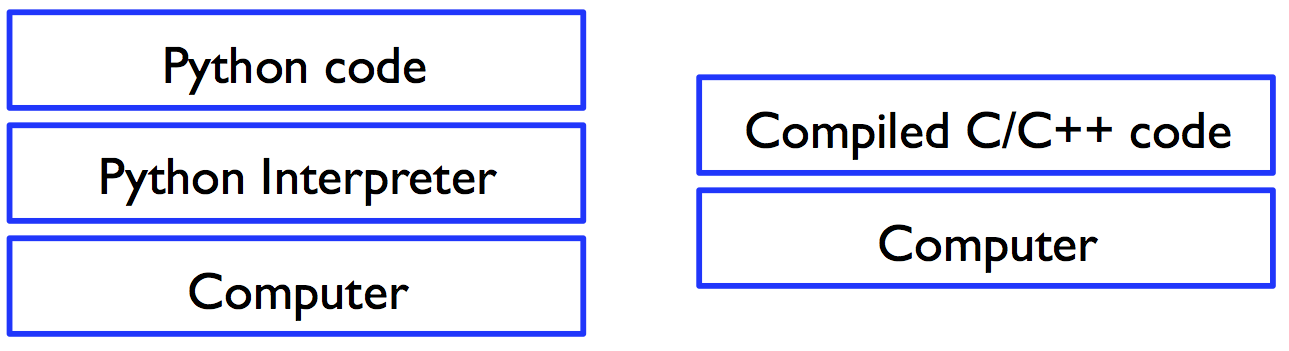
\includegraphics[scale=0.45]{fig/python-v-compiled.png}
\caption{\footnotesize The Python interpreter sits between the programmer's code and
the machine. In the case of a lower level language such as C++, the
programmer has direct control over memory management and more granular
control over data types. A knowledgeable programmer can take advantage
of the particular computer architecture they are using, alongside the
problem constraints, in order to more efficiently write code to solve
a task. This is harder with Python, wherein the code that the
programmer writes is first translated by the interpreter such that the
machine may understand it. We remark that of course C++ code also must
be translated to machine code, but that it ties in much closer to said
assembly code than Python.}
\end{figure}

\subsubsection{Runtime Performance: An Empirical Example}
Let's compute \(2^i\) for \(i \in [0,n)\). We can use the
\href{https://docs.python.org/3/library/timeit.html#basic-examples}{\texttt{timeit} module}.
Using lists, and from the command line
interface.

\begin{lstlisting}[language=bash,basicstyle=\small]
  $ python3 -m timeit --setup='L=range(1000)' '[i**2 for i in L]'
\end{lstlisting}

Equivalently, we can use the \texttt{\%timeit} magic command in an
IPython notebook.

\begin{lstlisting}[language=bash,basicstyle=\small]
  $ ipython
  In [1]: L = range(1000)
  In [2]: %timeit [i**2 for i in L]
\end{lstlisting}

What happens if we try the same operation using \texttt{numpy}? The
analogous operation to \texttt{range} in built-in Python is the
\texttt{arange} method in \texttt{numpy}. For integer arguments, the
two functions behave the same, but \texttt{numpy.arange} extends to
handling non-integer arguments.\footnote{The \texttt{range}
  sub-routine is designed to return \emph{indices} that can be used as
  subscript arguments when slicing an object, whereas the
  \texttt{numpy.arange} is a more generalized function which can take
  arbitrary boundary points and step-sizes.}

\begin{python}
  import numpy as np
  a = np.arange(1000)
  %timeit a**2
\end{python}

On my machine, the difference is about 300x.
We'll explore how \texttt{numpy} is able to achieve such
performance gains throughout the lecture. For now, let's continue to
explore how the module can not only allow our programs to execute
faster once built, but in fact \texttt{numpy} lets us write the more
concise code that is capable of a higher level of abstraction. 

\subsubsection{Programmer Productivity}
And even though Python is a high-level programming language, it's
still a general purpose one. I.e. it is not tailored to numerical or
scientific computing. Whence we \emph{do} have to write additional
code in order to abstract away commonly used operations in maths and
sciences.

E.g. let's add some 2D arrays. 
In Python, we could try and create a two-dimensional tabular data
structure using lists of lists. In order to facilitate something as
easy as ``adding'' two 2D-arrays together, we'd have to write our own
sub-routine, since the \texttt{+} operator performs
\emph{concatenation} on lists rather than element wise addition!

\begin{python}
def my_ones(nrows, ncols):
    """
    Create a matrix-like object of dimension nrows x ncols, with each
    element taking unit value.
    """
    A = []
    for r in range(nrows):
        A.append([])
        for c in range(ncols):
            A[r].append(1.0)
    return A

def matrix_add(A,B):
    """
    Create a new matrix-like object to store the result of adding
    input matrices A and B. We assume the matrices have identical
    dimension. The work required by the algorithm is proportional to
    the number of elements stored in the input matrices.
    """
    C = []
    for r in range(len(A)):
        C.append([])
        for c in range(len(A[r])):
            C[r].append(A[r][c] + B[r][c])
    return C

nrows, ncols = 3, 2
A = my_ones(nrows,ncols)
B = my_ones(nrows,ncols)
C = matrix_add(A,B)
\end{python}

What about with \texttt{numpy}? The operations are trivial to carry
out without defining our own data structures or sub-routines.
I.e. we can ``program faster''.

\begin{python}
nrows = 3
ncols = 2

A = np.ones((nrows,ncols))
B = np.ones((nrows,ncols))

C = A + B
\end{python}

Seems a lot easier to write. Let's check if we earned ourselves a performance again.
Suppose we have placed our definition of \texttt{my\_ones} into a
standalone file in our current working directory, which we call
\texttt{my\_module.py}. We may time the performance as
follows, using
\begin{lstlisting}[language=bash,basicstyle=\small]
  $ python3 -m timeit --setup='import my_module' 'my_module.my_ones(1000, 500)'
\end{lstlisting}

Alternatively, in an IPython notebook we may simply
write \texttt{\%timeit A = my\_ones(1000,500)}.
\texttt{numpy} is able to accomplish the analogous operation on my
machine approximately 200x faster. I.e. whereas the hand-rolled variant required
50 \emph{milliseconds} per loop, the \texttt{numpy} analogue below
requires only 200 \emph{microseconds} per loop.\footnote{There are 1,000
microseconds in a millisecond.}

\begin{lstlisting}[language=bash,basicstyle=\small]
  $ python3 -m timeit --setup='import numpy as np' 'np.ones((1000, 500))'
\end{lstlisting}

What about our add operation? In a IPython notebook, with \texttt{my\_ones} as per above.

\begin{python}[basicstyle=\footnotesize]
nrows = 1000
ncols = 500

A = my_ones(nrows,ncols)
B = my_ones(nrows,ncols)
%timeit C = matrix_add(A,B)

A = np.ones((nrows,ncols))
B = np.ones((nrows,ncols))
%timeit C = A + B
\end{python}

Again we see that \texttt{numpy} is orders of magnitude faster.

\paragraph{Object Overhead} The reason that our \texttt{list} of
\texttt{list}s was so much slower than \texttt{numpy} relates in part
to object overhead.

\begin{figure}[h]
\centering
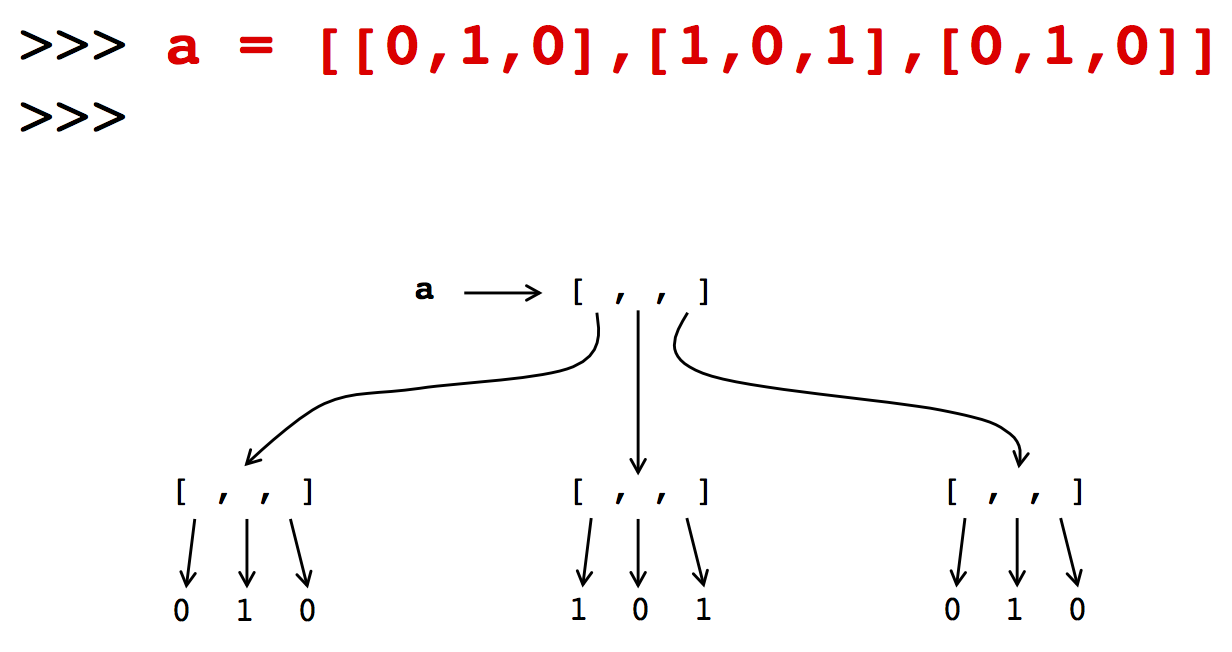
\includegraphics[scale=0.45]{fig/object-overhead.png}
\caption{Recall that objects in Python are references, and that a
  reference is simply a location in memory associated with a type and
  a value. If we create a \texttt{list} of \texttt{list}s to represent
  2D-tabular data, we end up with several layers of indirection. Part
  of the practical implication of having to jump around in memory in
  order to obtain data that ``should appear next to each other'' is
  that we realize many more
  \href{https://en.wikipedia.org/wiki/CPU_cache\#Cache_miss}{cache-misses}.}
\end{figure}

\subsection{Options for better performance}

Python is great for quick projects, prototyping new ideas, etc. but
what if you need better performance?
One option is to completely rewrite your program in something like
C or C++

\subsubsection{Python C API}
Python has a \href{https://docs.python.org/3/c-api/intro.html}{C API}
which allows the use of compiled modules.

\begin{figure}[h]
\centering
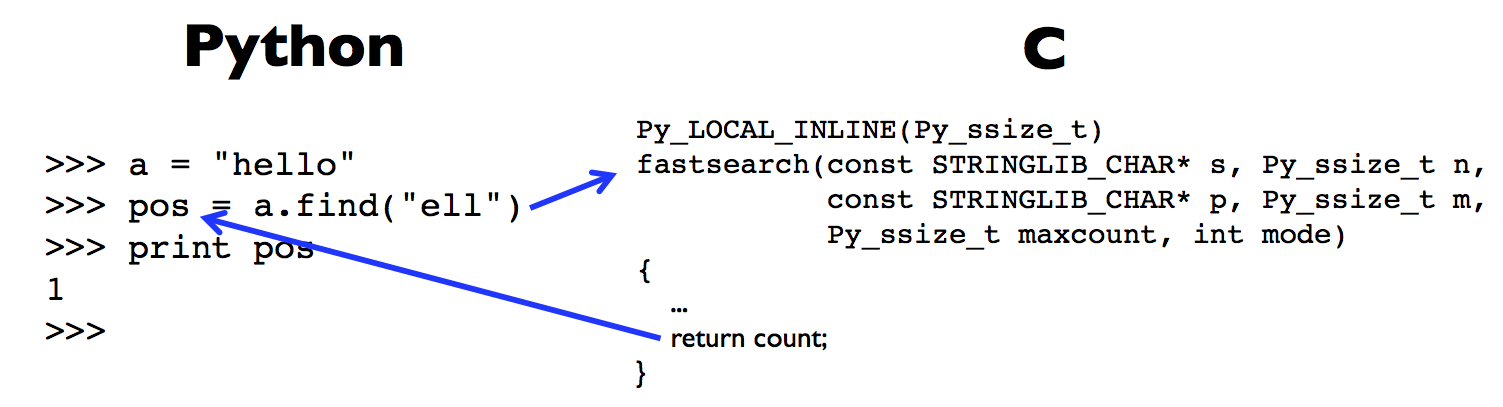
\includegraphics[scale=0.45]{fig/python-c-interface.png}
\caption{When we call the \texttt{str.find()} method, we're actually
  making a call to native C-code. What's happening here?
  Within the native C-code, we can
  include a Python module that gives us a way to write C modules which
  extend to being able to be used by the Python interpreter.}
\end{figure}

The actual implementation of \texttt{string.find()} can be viewed at:
\href{https://github.com/python/cpython/blob/master/Objects/stringlib/fastsearch.h}.

\subsubsection{Python compiled modules}

Python code in a \texttt{.py} file is actually executed in a hybrid
approach by a mix of the interpreter and compiled modules that come
with Python. See
\href{https://docs.python.org/3/tutorial/modules.html#compiled-python-files}{compiled
  python files}: the compilation doesn't make the code execute faster,
it just means the definitions in a script can be loaded faster into
memory (but once loaded, the complexity of each algorithm is the same).

\begin{figure}[h]
\centering
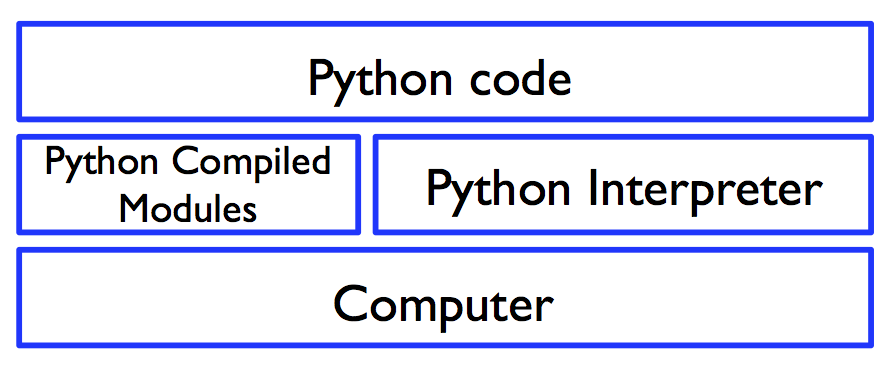
\includegraphics[scale=0.45]{fig/python-compiled-modules.png}
\caption{Perhaps closer to reality, the Python code we write sits atop
not only an interpreter but also additional compiled modules that we
import.}
\end{figure}

The same Python C API used by the developers of Python itself also
allows other programmers to develop and build their own compiled
extension modules.
These modules extend the functionality of Python with high performance
implementations of common operations.

\paragraph{Commonly Used Modules: NumPy, SciPy, Matplotlib}

\begin{itemize}
\item
  NumPy - multidimensional arrays and fundamental operations on them.
\item
  SciPy - Various math functionality (linear solvers, FFT, optimization,
  etc.) utilizing NumPy arrays.
\item
  matplotlib - plotting and data visualization.\footnote{None of these packages seek to clone (all of) MATLAB, if you want that try
something like GNU Octave.}
\end{itemize}

\begin{figure}[h]
\centering
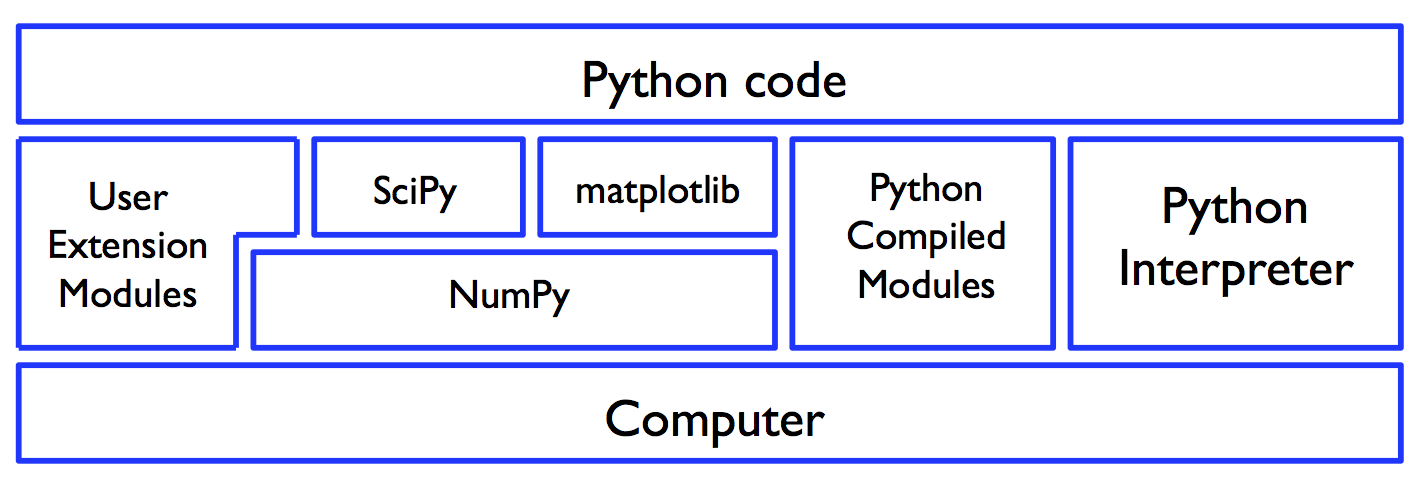
\includegraphics[scale=0.45]{fig/python-stack.png}
\caption{A schematic of how Python code sits on top of an entire set
  of Pythonic tools, which ultimately relay human-readable language instructions into
  machine-code.}
\end{figure}

\subsection{NumPy}
At its core, \texttt{numpy} provides an
\href{https://docs.scipy.org/doc/numpy/reference/arrays.html}
{$n$-dimensional numeric array object}:

\begin{python}
import numpy as np
a = np.array([7, 42, -3])
print(a)                     # Prints out: "array([ 7, 42, -3])"

a[1] = 19                    # Numeric arrays support item assignment.
a                            # Corresponding element is modified.
\end{python}

\paragraph{Arrays are \emph{not} Lists}
For performance reasons, \texttt{numpy.array}s do not store
heterogeneous data.
Instead, \texttt{numpy.array} is said to be
\textbf{homogeneous}: each element is of exactly the same type and hence
requires the same amount of storage in memory, and further each block
of memory (i.e. element) can be interpreted in an identical
fashion.\footnote{Note that although the types must be homogeneous, they need
not be atomic, e.g. we can store data strucutures within an
\texttt{array}.}

\begin{python}
  a[0] = "hello"    # ValueError: invalid literal for int().
  a.append(0)       # AttributeError: numpy.ndarray object has no attribute 'append'.
\end{python}

Further, the \textbf{size is fixed}, i.e.~you \textbf{can't append or remove}.

\subsubsection{Data Types}
Numerical analysts must pay close attention to their data types, and
be wary of an algorithm's
\href{https://en.wikipedia.org/wiki/Numerical_stability}{numerical
  stability}. To that end, \texttt{numpy} allows the programmer to
specify exactly what data type they are choosing to store in
underlying elements of the array.

\paragraph{Integers}
Can be stored in 8, 16, 32, and 64 bit variants, and additionally they
can be either signed or unsigned. We specify these by
e.g. \texttt{np.int8}, \texttt{np.uint8}. For more information, see
\href{https://docs.scipy.org/doc/numpy/reference/arrays.dtypes.html}
{\texttt{dtype} documentation}.

\paragraph{Floating Point}
Can be stored in either 32, 64, or 128 bit variants (all signed). We
specify these by e.g. \texttt{np.float32}, \texttt{np.float64}, etc.

Complex numbers,
strings, and Python object \emph{references} also supported by \texttt{numpy}.

\paragraph{Data Type Examples}
\begin{python}
a = np.array([ 7, 19, -3], dtype=np.float32)

a[0] = a[0]/0.     # RuntimeWarning: divide by zero encountered in true_divide. Returns inf.

b = np.array([4, 7, 19], dtype=np.int8)
b[0] = 437         # Example of overflow and wraparound. Range is [-128, 127]
\end{python}

Note that we can witness the wraparound behavior for ourselves quite
clearly as follows.

\begin{python}
  b[0] = 127       # Print and inspect data; stored as expected.
  b[0] = b[0] + 1  # Attempt to increment by unit value.
  print(b)         # Note that first element now -128.
\end{python}

\subsubsection{Multidimensional Arrays}
Arrays can have multiple dimensions called \texttt{axes}.
The number of \emph{axes} is called the \texttt{rank}.
These terms come from the NumPy community and should \emph{not be confused
with linear algebra terms} for \emph{rank}, etc.

\begin{python}
# Create a two-dimensional array. I.e. two rows, each with three elements.
a = np.array([(7, 19, -3), (4, 8, 17)], dtype=np.float64)

# Array 'a' has a slew of attributes (and methods) associated with it.
a.ndim      # Returns the number of dimensions or axes: 2
a.dtype     # Returns the data type stored:             dtype('float64')
a.shape     # Returns the extents of each dimension:    (2, 3)
a.size      # Returns the number of elements:           6
\end{python}

\subsubsection{Internal Representation}
How can we think about the internal representation of a
\texttt{numpy.array} object? The object itself contains
\emph{attributes} (some shown above), alongside a reference to a
fixed-width sequence of bits in memory which describe the underlying data.

\begin{figure}[h]
\centering
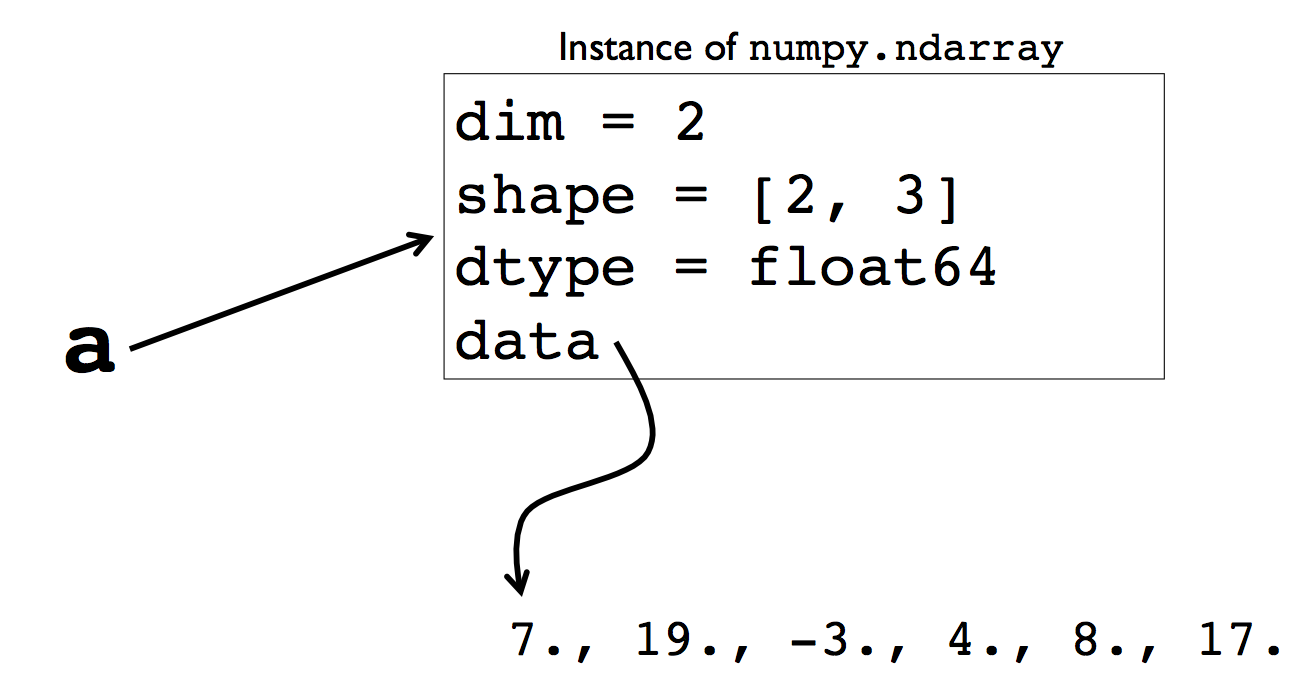
\includegraphics[scale=0.45]{fig/numpy-representation.png}
\caption{fig}
\end{figure}

Since each element of the array is of the same type, and each requires
the same amount of storage, we can know how to \emph{slice} into a
particular element in our array in constant time.

\subsubsection{Creating Arrays}

\begin{python}
a = np.empty((3,3))   # A 3x3 matrix of *un-initialized* entries, not necessarily zeros!
a = np.zeros((3,3))   # A 3x3 matrix of *zero-initialized* entries.
a = np.ones((3,3))    # A 3x3 matrix of *unit-unitialized* entries.

a = np.eye(3)         # A 3x3 identity matrix.

a = np.arange(9, dtype=np.float64)               # A 1D sequence of integers 0-8.
a = np.arange(9, dtype=np.float64).reshape(3,3)  # A 2D sequence of integers 0-8...
                                                 # ... arranged in a 3x3 layout.
\end{python}

\subsubsection{Reading data from a file}

\begin{lstlisting}[language=bash]
$ cat numbers.txt
7. 19. -3.
4. 8. 17.
\end{lstlisting}

\begin{python}
a = np.loadtxt('numbers.txt', dtype=np.float64)
a = a + 1      # Element-wise addition!
np.savetxt('numbers2.txt', a)
\end{python}

\subsubsection{Remove single dimension entry}

\begin{python}
a = np.arange(3)   # Think of this like a 1D row-vector.
a.shape            # (3,)
b = np.arange(3).reshape(3,1)  # We now realize a 2D-array: 3x1.
print(b.shape)                 # Returns (3, 1)
b = np.squeeze(b)              # Removes 1D entries from the shape of an array.
print(b)                       # Now a 1D row-vector, just like 'a'.
print(b.shape)                 # Returns (3,)
\end{python}

Perhaps another informal way of thinking about this function: it removes any
``nested, superfluous'' dimensions.  Suppose we create a 3D array with
six elements as follows.

\begin{python}
# Recall: arange simply returns an 'array' with 'range' evenly-spaced values.
a = np.arange(6).reshape((3, 1, 2))

# a[i] peels off the first dimension (i.e. returns an ndarray with shape (1, 2).
# but the second axis has only a single element, i.e. a[i][1] is INVALID. 
# Might as well drop this dimension via squeeze.
\end{python}

\subsubsection{Array Operations}

\begin{python}
a = np.arange(9, dtype=np.float64)   # Store values 0-8 inclusive.
a[3:7]                               # Returns values 3-6 inclusive.

a[3:7] = 0                           # Assign value zero to be referenced 
                                     # by the fourth and up till but
                                     # excluding the eigth element.
# Elementwise rescaling.
2*a
a*a

# Vector operations are supported "right out of the box".
sum(a)
min(a)
max(a)
\end{python}

\paragraph{Don't Reinvent the Wheel} It can be tempting for newer
programmers to implement everything from scratch. This leads to not
only more code to maintain but programs which are not as
performant. Consider implementing a procedure for calculating the 
\href{https://en.wikipedia.org/wiki/Norm_(mathematics)\#Euclidean_norm}
{Euclidean norm} of a vector.

\begin{python}
a = np.arange(9, dtype=np.float64)   # Store values 0-8 inclusive.

# Bad idea.
import math
total = 0.
for n in range(len(a)):
    total += a[n]*a[n]

math.sqrt(total)

math.sqrt(np.dot(a,a))  # Better idea: 1-liner and more performant than interpreted loop.
np.linalg.norm(a)       # Best idea! (Not necessarily faster still, just more concise).
\end{python}

The last expression is both the most concise and at least as
performant as any other.

\subsubsection{Speed of Array Operations}

Some of the overloaded operators (e.g. \texttt{min}, \texttt{max},
\texttt{sum}, etc.) work albeit slowly.
In an IPython notebook:
\begin{python}
%timeit total = sum(np.ones(1000000,dtype=np.int32))
%timeit total = np.sum(np.ones(1000000,dtype=np.int32))
\end{python}

Same data, same input. Using built-in \texttt{sum} requires (on my
machine) an average of 700 microseconds per loop, whereas the
corresponding \texttt{numpy.sum} is about 35x faster, requiring only
20 microseconds per loop. Why is there such a big difference?

Loops you write in Python will be executed by the interpreter.
Calling NumPy function or methods of the array object will invoke high
performance implementations of these operations, which can be
specialized to operate on homogeneous data.

\subsubsection{Matrix Operations}

\begin{python}
a = np.arange(9, dtype=np.float64).reshape(3,3)  # 3x3 matrix, row-major order.

# Basic operations on a single matrix.
a.transpose()
np.trace(a)

# Be careful with "matrix" multiplication!
a*a           # Naive element wise multiplication.
np.dot(a,a)   # True matrix-matrix multiplication.
a @ a         # Equivalently: new matrix multiply operator in Python 3.5.
\end{python}

Note that if we use \texttt{ndarray}, then the \texttt{*} operator is
applied elementwise, whereas if we have a \texttt{matrix} we get the
benefit of being able to use a true matrix-multiply.

\subsubsection{Array vs Matrix}
NumPy has a dedicated matrix class
However, the matrix class is not as widely used and there are subtle
differences between a 2D array and a matrix.
It is highly recommended that you use 2D arrays for maximum
compatibility with other NumPy functions, SciPy, matplotlib, etc.
See here for more details:
\url{http://www.scipy.org/NumPy_for_Matlab_Users}.

\subsubsection{References to an Array}

\begin{python}
a = np.arange(9, dtype=np.float64).reshape(3,3)
b = a         # Recall: assignment sets up a reference.
b[0,0] = 42   # For the ndarray referred by b, modify "first" element.
b             # Of course, ndarray reffered to by 'b' has changed.
a             # Hopefully not a surprise: 'a' referred to the same object...
\end{python}

\paragraph{Array slices and references}

\begin{python}
a = np.arange(9, dtype=np.float64)
b = a[2:7]    # Create a reference to the underlying data, elements 3:7 inclusive.
b[2] = -1     # When we modify this data... (third elem in 'b', i.e. fifth elem in 'a')
a             # ... 'a' also refers to the same data. Whence 'a' mutated.
\end{python}

\hypertarget{array-copies}{%
\subsubsection{Array copies}\label{array-copies}}

\begin{python}
a = np.arange(9, dtype=np.float64)
b = a.copy()       # Set up a reference to a *copy* of the array.
b[4] = -1          # Mutating 'b' doesn't affect object referred by 'a'.
a
\end{python}

\subsubsection{Universal functions (ufunc)s}

Within \texttt{numpy}, there is a subclass
\href{https://docs.scipy.org/doc/numpy-1.15.1/reference/ufuncs.html#universal-functions-ufunc}
{\texttt{ufunc}} which operate on \texttt{ndarray}s in an elementwise fashion.
\begin{python}
import numpy
import math
a = np.arange(9, dtype=np.float64)
math.sqrt(a)   # Error: only size-1 arrays can be converted to Python scalars.
np.sqrt(a)     # Works: square root operator is applied element-wise.
\end{python}

We can think of \href{https://docs.scipy.org/doc/numpy-1.15.1/reference/ufuncs.html#universal-functions-ufunc}{\texttt{ufunc}}s as a vectorized wrapper for a function
which usually operates on a single datum at a time (typically scalars).

\subsubsection{Beyond Just Arrays}
\begin{itemize}
\item
  NumPy has some support for some useful operations beyond the usual
  vector and matrix operations:

  \begin{itemize}
  \item
    Searching, sorting, and counting within arrays
  \item
    FFT (Fast Fourier Transform)
  \item
    Linear Algebra
  \item
    Statistics
  \item
    Polynomials
  \item
    Random number generation
  \end{itemize}
\item
  SciPy has largely replaced much of this functionality, plus added much
  more
\end{itemize}

\subsubsection{Warning}
\begin{itemize}
\item
  Once you start making use of extension modules such as NumPy, SciPy,
  etc. the chances of code ``breaking'' when you run it on different
  machines goes up significantly
\item
  If you do some of your development on machines other than corn (which
  isn't the model we advise) you may run into issues
\end{itemize}

\subsubsection{Further Reading}
\begin{itemize}
\item
  MATLAB users: \url{http://www.scipy.org/NumPy_for_Matlab_Users}
\item
  NumPy tutorial at: \url{http://www.scipy.org/Tentative_NumPy_Tutorial}
\item
  Official docs at: \url{http://docs.scipy.org/}
\end{itemize}

\end{document}
